\documentclass[a4paper,12pt]{article}

\title{Exercise 4: Distance to the green box}
\author{Group 6:\\Niels\\Troels\\Mark\\Kristian}

\usepackage[T1]{fontenc}
\usepackage{lmodern}
\usepackage[utf8]{inputenc}
\usepackage[british]{babel}
\usepackage{microtype}
\usepackage{underscore}
\usepackage{amsmath}
\usepackage{graphicx}
\usepackage[hidelinks]{hyperref}

\setlength{\parskip}{1ex}
\setlength{\parindent}{0pt}
\setlength{\parfillskip}{30pt plus 1 fil}

\begin{document}

\maketitle

\section{Distance from one image}

\subsection{Estimating the field of view}

We need to know the FOV of our camera to be able to measure the distance to an
object with just one image.

See our program \texttt{findfov.cc} for the implementation.  It detects a green
box and uses its height in pixels in the image to calculate the field of view in
degrees.

Let
\begin{itemize}
\item $h_b$ be the known height of a box in centimeters;
\item $d$ be the known distance to the box;
\end{itemize}

and let
\begin{itemize}
\item $h_t$ be the total height of the image;
\item $v_c$ be the known vertical resolution of the camera in pixels;
\item $v_b$ be the measured vertical size of the box in pixels; and
\item $f$ be the field of view.
\end{itemize}

Then we consider the triangle with sides $a$, $b$, and $c$ and angles $A$, $B$,
and $C$, and calculate $f$:

\begin{align*}
  h_t &= \frac{v_c}{v_b} \cdot h_b\\
  a &= \frac{h_t}{2}\\
  b &= d\\
  c &= \sqrt{a^2 + b^2}\\
  A &= \arcsin \frac{a}{c}\\
  f &= 2 \cdot A
\end{align*}

We measured the FOV of our camera to be 39.5 dregrees.


\subsection{Measuring the distance to the box}

See our library function \texttt{distance_two_pictures} in \texttt{cam.cc} for
the implementation.

Let
\begin{itemize}
\item $h_b$ be the known height of the box in centimeters;
\item $v_c$ be the known vertical resolution of the camera in pixels;
\item $f$ be the known field of view;
\end{itemize}

and let
\begin{itemize}
\item $v_b$ be the measured vertical size of the box in pixels; and
\item $d$ be the distance to the box.
\end{itemize}

Then we consider the triangle with sides $a$, $b$, and $c$ and angles $A$, $B$,
and $C$, and calculate $d$:

\begin{align*}
  A &= \frac{f}{2}\\
  a &= \frac{h_b \cdot \frac{v_c}{v_b}}{2}\\
  c &= \frac{a}{\sin A}\\
  b &= c \cdot \cos A\\
  d &= b.
\end{align*}


\section{Distance from two images}

See our library function \texttt{distance_height_known} in \texttt{cam.cc} for
the implementation.

Let

\begin{itemize}
\item $d_b$ be the known travelled distance from the first position to the
second position; and
\end{itemize}

and let

\begin{itemize}
\item $v_{b_1}$ be the measured vertical size of the box in pixels from the
starting point;
\item $v_{b_2}$ be the measured vertical size of the box in pixels after having
travelled $d$ centimeters; and
\item $d$ be the distance to the box from the second position.
\end{itemize}

Then we use the relationship between the measured sizes to calculate $d$:

\begin{align*}
  d &= d_b * \frac{v_{b_1}}{v_{b_2} - v_{b_1}}
\end{align*}


\section{Detection of green box}

We're using the same algorithm as in our previous assignment, although with minor
tweaks in its magic constants.
\section{Test-program}
To calculate the distances we first wrote a test-program to collect the test results. The robot-program starts 250 centimeters from a green piece of paper and runs until it's 75 centimeters away. The program runs in a loop where it first centers the robot such that the green piece of paper is in the middle of the camera's picture. Once it's centered it takes ten pictures and run 25 centimeters closer to the paper. This loop repeats until the last measurements are made. 
We save all measurements in a Matrix(List List). We then use the two different techniques to calculate the distances and write them to separate txt files.
We this use a python-script (reg.py) to make a fit on the data, calculate the variance, and plot the data.
\subsection{Data}
The first graph represents the calculated fit using the field-of-view technique.
\begin{figure}[!h]
\centering
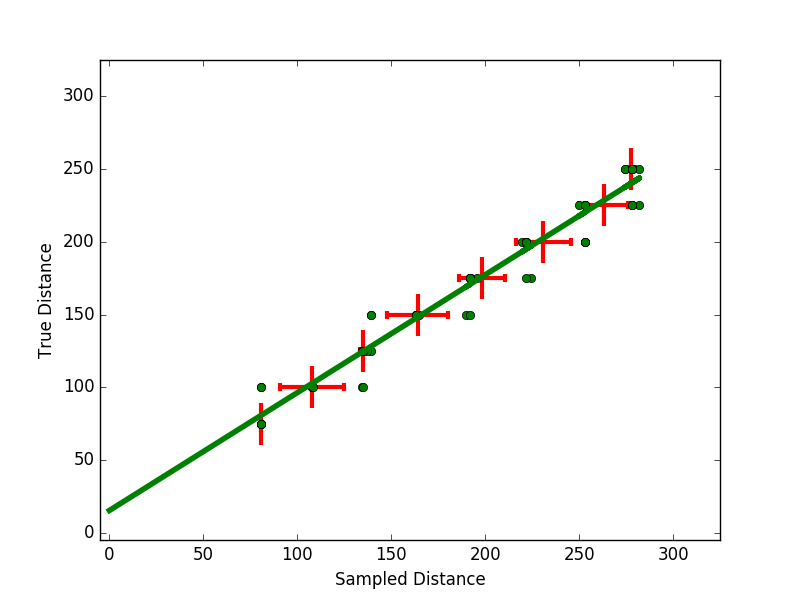
\includegraphics[scale=0.65]{fov}
\caption{Regression of sample data from field-of-view technique}
\label{fig:fov}
\end{figure}
We have made a rough selection of removed outliers, yet we still see that the variance is high. The fitted regression gave us: $0.81005588729\cdot x + 15.2963279573$. This isn't very good. We would hope the the value $\sim$15.3 would be closer to 0 and the $\sim$0.81 would be closer to 1. If this was the case the method could be proper to estimate the real distances.
\\

The second graph represents the calculated fit using the two-pictures-technique.
\begin{figure}[!h]
\centering
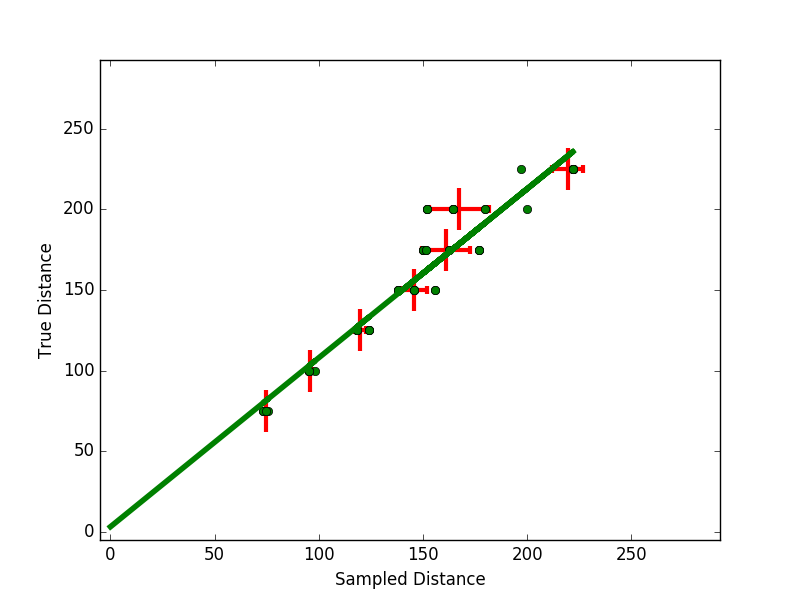
\includegraphics[scale=0.75]{box}
\caption{Regression of sample data from two-pictures-technique}
\label{fig:box}
\end{figure}

Here we see that the variance is a bit lower giving us a somewhat better result. The fitted regression gave us: $1.04749081738\cdot x + 3.20182889525$. This is a lot closer to the expected values of 1 and 0, which could indicate that the two-pictures technique gives us a better better result.


\end{document}
